\documentclass[11pt]{amsbook}

\usepackage{../HBSuerDemir}

\begin{document}

% ++++++++++++++++++++++++++++++++++++++
\hPage{b1p2/304}
% ++++++++++++++++++++++++++++++++++++++

\begin{multicols}{2}
	\begin{equation}
    \{(r_1, r_2): r_1 + r_2 = 2a\}
    \label{eq:b1p2_304_firstEquation}
  \end{equation}

	\begin{equation}
    \{(r_1, r_2): |r_1 - r_2| = 2a\}
    \label{eq:b1p2_304_secondEquation}
  \end{equation}
\end{multicols}
\begin{multicols}{2}
	\begin{equation}
    \{(r_1, r_2): r_1 \cdot r_2= \ell^2\}
    \label{eq:b1p2_304_thirdEquation}
  \end{equation}

	\begin{equation}
    \{(r_1, r_2): r_1 : r_2 = k \neq 1\}
    \label{eq:b1p2_304_fourthEquation}
  \end{equation}
\end{multicols}

\noindent represent respectively an ellipse, a hyperbola and a circle
(circle of APOLLONIUS); as to \refeq{eq:b1p2_304_thirdEquation}, it represents
a curve called \textit{oval to CASSINI} including the curve named
\textit{lemniseate of BERNOULLI}.\\

% =======================================
\subsubsection{Distance between two points}
\label{subsubsec:DistanceBetweenTwoPoints}

The distance $d = d(P_1, P_2)$ between two given points
$P_1(\theta_1, r_1), P_2(\theta_2, r_2)$ is obtained by the use of cosine law
applied to the triangle $O P_1 P_2$:

\begin{minipage}{0.55\textwidth}
	\[
		d^2 = r_1^2 + r_2^2 - 2 r_1 r_2 \cos(\theta_2 - \theta_1)
	\]
	where $\cos(\theta_2 - \theta_1) = \cos(\theta_1 - \theta_2)$
\end{minipage}%
\begin{minipage}{0.45\textwidth}
	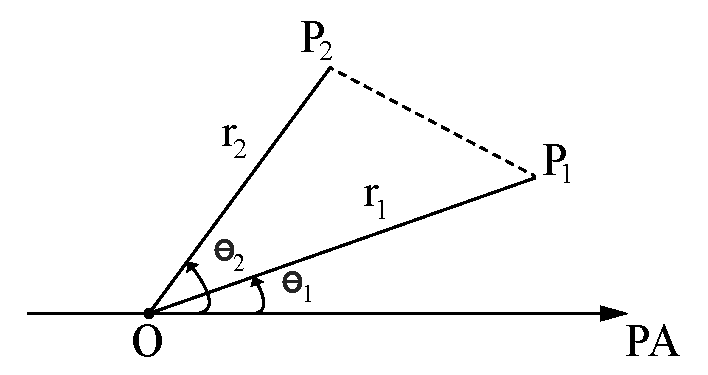
\includegraphics[width=1\textwidth, keepaspectratio]{images/b1p2-304-fig01}
\end{minipage}

It is valid for any determinations of $P_1, P_2$, since the right hand side
remains unaltered when $\theta_1$ is replaced by $\theta_1 + \pi$ and
$r_1$ by $-r_1$\\

\begin{exmp}
	Find the distance between the given pair of points:

	\begin{multicols}{2}
		a) $A(\frac{\pi}{3},-2),\ B(\frac{\pi}{6},4)$

		b) $C(-\frac{\pi}{4},3),\ D(\frac{3\pi}{4},-3)$
	\end{multicols}

	\begin{hSolution}
		\begin{flalign*}
			\text{a)}\ d^2 &= |AB|^2 = 4 + 16 - 2 (-2) (4) \cos(\frac{\pi}{3} - \frac{\pi}{6})&\\
			               &= 20 + 16 \cos \frac{\pi}{6} = 20 + 8 \sqrt{3}&\\
			               & \indent d = |AB|=\sqrt{20+8 \sqrt{3}}&\\
			\text{b)}\ d^2 &= |CD|^2 = 9 + 9 - 2 (3) (-3) \cos(\frac{3\pi}{4} + \frac{\pi}{4})&\\
			               &= 18 + 18 \cos \pi = 0&\\
			               & \indent d = 0\ \text{(explain this result!)}
		\end{flalign*}
	\end{hSolution}
\end{exmp}

% =======================================================
\end{document}
